\documentclass{article}
\usepackage{nips15submit_e,times}
\usepackage{hyperref}
\usepackage{url}
\usepackage{amsmath}
\usepackage{amsfonts,amssymb}
\usepackage{graphicx}

\title{Weekly Report(Aug.6,2018-Aug.12,2018)}

\newcommand{\fix}{\marginpar{FIX}}
\newcommand{\new}{\marginpar{NEW}}

\begin{document}

\maketitle

\begin{abstract}
  In this week, I have finished \textbf{Machine learning} on coursera, but haven't finished those exercises yet. Besides, I'm making an endeavour to train the the object detection network \textbf{SSD} but failed for numerous inexplicable problems, therefore I didn't write them down this week.
\end{abstract}

\section{Work done in this week}
\subsection{Clustering}
\subsubsection{K$-$means algorithm}
For unsupervised learning, how can we figure out the inner structure of those data? We can do clustering using K$-$means algorithm:\\
Input:
\begin{description}
  \item[-] $K$(number of clusters)
  \item[-] Training set ${x^{(1)}, x^{(2)}, \ldots, x^{(m)}}$
\end{description}
$x^{(i)} \in \mathbb{R}^n$(drop $x_0 = 1$ convention)\\
Randomly initialize $K$ cluster centroids $\mu_1, \mu_2, \ldots, \mu_K \in \mathbb{R}^n$\\
Repeat\{\par
\hspace{1cm} $i = 1$ to $m$\par
\hspace{2cm}$c^{(i)}$ := index (from 1 to $K$) of cluster centroid closest to $x^{(i)}$\par
\hspace{1cm}for $k = 1$ to $K$\par
\hspace{2cm}$\mu_k$ := average (mean) of points assigned to cluster $k$\\
\}

\subsubsection{Optimization objective}
Cost function:\[J(c^{(1)}, \ldots, c^{(m)}, \mu_1, \ldots, \mu_K) = \frac{1}{m}\sum\limits_{i=1}^{m}\|x^{(i)} - \mu_{c(i)}\|^2\]
Our goal is to minimize the cost function. As we know, the first loop minimizes what $c^{(i)}$ costs, and the second loop minimizes what $\mu_i$ costs. Therefore, the cost
decreases every iteration. Otherwise, there must be some errors.

\subsubsection{Random initialization}
To avoid local minimum, we always run K$-$means algorithm for many times, and do random initialization every time.\\
For $i = 1$ to $100$ \{\par
$\hspace{2cm}$Randomly initialize K$-$means.\par
$\hspace{2cm}$Run K$-$means. Get $c^{(1)}, \ldots, c^{(m)}, \mu_1, \ldots, \mu_K.$\par
$\hspace{2cm}$Compute cost function(distortion) $J(c^{(1)}, \ldots, c^{(m)}, \mu_1, \ldots, \mu_K)$.\par
\}\\
Pick clustering that gave lowest cost $J(c^{(1)}, \ldots, c^{(m)}, \mu_1, \ldots, \mu_K)$.

\subsection{Dimensionality Reduction}
PCA is a common algorithm for dimensionality reduction.
Reduce data from $n-$dimensions to $k-$dimensions\\
Compute "covariance matrix":\[\sum = \frac{1}{m}\sum\limits_{i=1}^n(x^{(i)})(x^{(i)})^T\]
Compute "eigenvectors" of matrix $\sum$:\[[U, S, V] = \text{svd(Sigma)};\]
We get:\[U = \left[
               \begin{array}{cccc}
                 | & | &   & | \\
                 u^{(1)} & u^{(2)} & \cdots & u^{(n)} \\
                 | & | &   & | \\
               \end{array}
             \right] \in \mathbb{R}^{n \times n}
\]
After mean normalization and optionally feature scaling:\[\text{Sigma} = \frac{1}{m}\sum\limits_{i=1}^m(x^{(i)})(x^{(i)})^T\]
[U, S, V] = svd(Sigma);\\
Ureduce = U(:, 1:k);\\
z = Ureduce'*x;\\
Typically, choose $k$ to be smallest value so that \[\frac{\frac{1}{m}\sum_{i=1}^m\|x^{(i)} - x_{approx}^{(i)}\|^2}{\frac{1}{m}\sum_{i=1}^m\|x^{(i)}\|^2} \leq 0.01\]
So "99\%" of variance is retained.

\subsection{Anomaly detection}
\begin{enumerate}
  \item Choose features $x_i$ that might be indicative of anomalous examples.
  \item Fit parameters $\mu_1, \ldots, \mu_n, \sigma_1^2, \ldots, \sigma_n^2$
        \[\mu_j = \frac{1}{m}\sum\limits_{i=1}^mx_j^{(i)}\]
        \[\sigma_j^2 = \frac{1}{m}\sum\limits_{i=1}^m(x_j^{(i)} - \mu_j)^2\]
  \item Given new example $x$, compute $p(x)$:
        \[p(x) = \mathop{\Pi}\limits_{j=1}^np(x_j;\mu_j,\sigma_j^2) = \mathop{\Pi}\limits_{j=1}^n\frac{1}{\sqrt{2\pi}\sigma_j}\text{exp}(-\frac{(x_j - \mu_j)^2}{2\sigma_j^2})\]
\end{enumerate}
Anomaly if $p(x) < \varepsilon$.

\subsection{Large scale machine learning}
\subsubsection{Stochastic gradient descent}
To see whether a large set of data is valuable, we can draw the learning curve. If we has to use a large set of data, stochastic gradient descent is a good choice. We define cost function:\[cost(\theta,(x^{(i)},y^{(i)})) = \frac{1}{2}(h_{\theta}(x^{(i)}) - y^{(i)})^2\]
\begin{enumerate}
  \item Randomly shuffle dataset.
  \item Repeat\{\par
        $\hspace{1cm}$for i = 1:m\{\par
        $\hspace{2cm}$$\theta_j:=\theta_j-\alpha(h_\theta(x^{(i)})-y^{(i)})x_j^{(i)}$\par
        $\hspace{2cm}$(for j = 0:n)\par
        $\hspace{1cm}$\}\\
  \}
\end{enumerate}

\subsubsection{Mini--batch gradient descent}
Say $b = 10, m = 1000$.\\
Repeat\{\par
$\hspace{1cm}$for $i = 1,11,21,31,\ldots,991$\{\par
$\hspace{2cm}$$\theta_j := \theta_j - \alpha\frac{1}{10}\sum\limits_{k=i}^{i+9}(h_{\theta}(x^{(k)}) - y^{(k)})x_j^{(k)}$\par
$\hspace{2cm}$(for every $j=0,\ldots,n$)\par
$\hspace{1cm}$\}\\
\}

\subsubsection{Map$-$reduce and data parallelism}
We can assign some mini dataset to a few computers, then combine those results.
\begin{center}
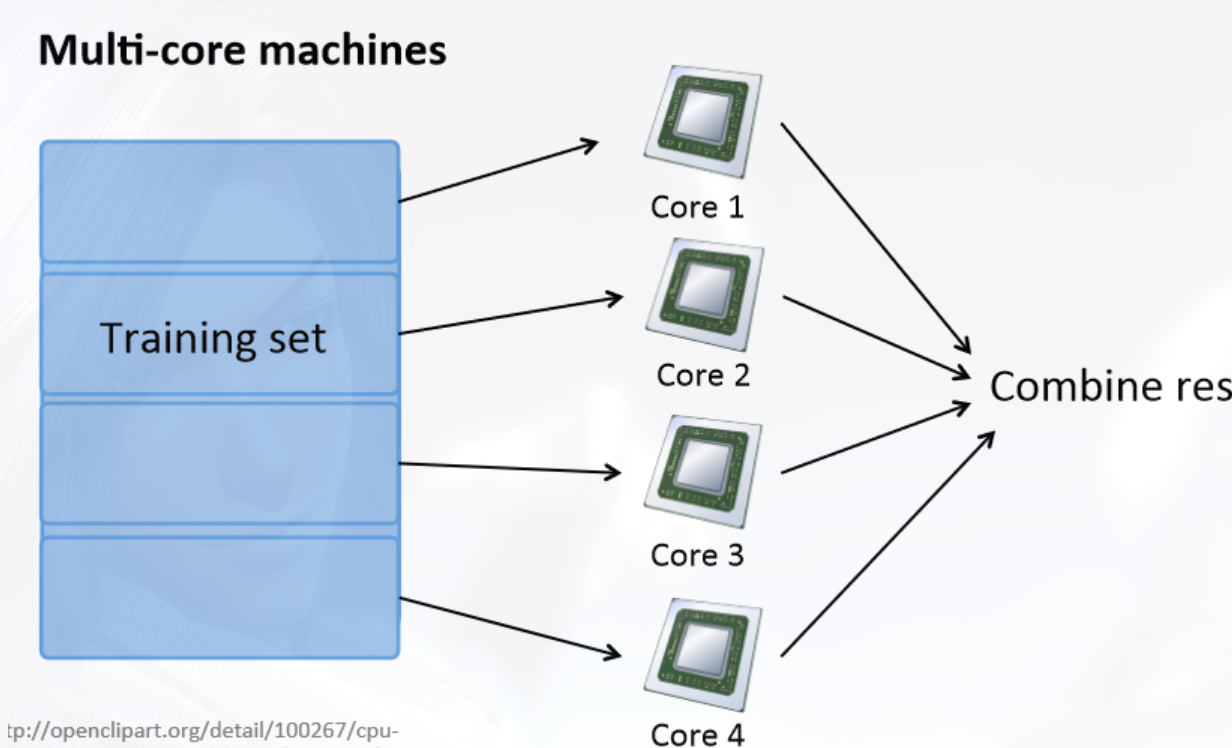
\includegraphics[scale=0.3]{1.png}
\end{center}
After finishing it, I still can't fully understand some algorithms and even forgot some contents learned earlier, which I think is not very efficient. Thus, I plan to take one or two weeks to review it and learn deeper about it. Are there any other useful references for machine learning?
\section{Plans for Next Week}
\begin{enumerate}
  \item Review \textbf{Machine Learning}.
  \item Finish my mathematical modeling assignment.
  \item Learn Lecture1, Lecture2, Lecture3 of \textbf{CS231n}.
  \item Keep on training \textbf{SSD}, and train other detection networks if possible.
\end{enumerate}

\end{document}
